\chapter[Implementation]{Implementation} \label{ch:implementation}

\section{Introduction}
Based on the evaluation carried out in \autoref{sec:consideredtech} the \acrlong{spa} was implemented with Vue and Nuxt. To give the reader a better understanding of how the application was built, the first few sections of this chapter will discuss which additional tools and functionalities Nuxt provides, how Vue is used and how \acrfull{soc} is achieved. Later sections which describe the specific implementation of UI elements do that from a functionality-based perspective and do not go into the specifics of CSS classes used, as these are described in depth in the Bulma documentation. It is enough for the reader to have a basic understanding of HTML and CSS.

\section{Nuxt.js}
Nuxt's primary use case is to provide \acrlong{ssr} for Vue-based applications. It also advertises itself as a framework which "presets all the configuration needed to make your development of a Vue.js application enjoyable" \cite{Nuxtjs:online}. While this blurry description is not very meaningful on its own, it indicates that Nuxt pre-configures certain parts of a Vue application. The most important of which are: \acrlong{ssr}, automatic setup of routing and store management.

\subsection{Rendering modes}
Nuxt offers three rendering modes: \acrshort{ssr}, "Prerendering" and "Single Page Application". For descriptions of the first two please see \autoref{sub:seo}. The "Single Page Application" mode does not offer server-rendering capabilities while still pre-configuring routing and state management. This mode is especially useful for applications that require users to be authenticated before being able to use them. The reason why is simple: \acrlong{ssr} can only improve the SEO ranking of a page if crawlers are able to look at the full contents of it. Fully implementing \acrshort{ssr} for an application that only shows a login form would therefore be pointless. 

Then why should this project use Nuxt, which is primarily used for \acrshort{ssr} if the application cannot even profit from it because authentication prevents crawlers from seeing anything but a login form? The answer is because 1) state management and routing are auto-configured as well and 2) because in the future, the frontend might expose parts of the system in a publicly accessible way without the need of authentication. By using Nuxt from the beginning, the transition to this is much easier.

\subsection{Usage}
When using Nuxt, different folders contain different parts of the frontend application. Behind the scenes, Webpack - one of the most popular bundler tools consolidates, minifies, transforms and transpiles the code of these folders into browser-readable plain JavaScript code. 

\begin{table}
    \begin{tabularx}{\linewidth}{|l|X|}
        \hline
        \textbf{Folder} & \textbf{Description} \\
        \hline
        assets & contains un-compiled assets such as images, global css or fonts  \\
        \hline
        components & contains reusable Vue Single File Components \\
        \hline
        layouts & contains Vue files that define the applications theme \\
        \hline
        middleware & defines files which are run before a route changes, e.g check if user is authenticated before redirecting \\
        \hline
        pages & contains the pages of the application, Nuxt automatically creates routes corresponding to a page's name \\
        \hline
        plugins & contains plain JavaScript files which are run before instantiating the application, e.g used for inject adding an internationalization plugin \\
        \hline
        static & files in this is directory are directly mapped to server root and are not compiled or renamed in any way, e.g robots.txt \\
        \hline
        store & contains Vuex store files, every file added in this directory is automatically mapped to the global store \\
        \hline
        nuxt.config.js & contains the Nuxt configuration for the application, e.g which plugins and middleware to use\\
        \hline
        package.json & is not Nuxt specific but added by npm and contains application dependencies and scripts \\
        \hline
    \end{tabularx}
    \caption{Nuxt Folder Structure}
    \label{table:filestructure}
\end{table}

Typically, functional components are defined inside the components folder. These components might include other components in order to compose more complex architectures. Pages and layouts are also nothing more than Vue components, however, they are used in very specific ways. The file structure of the pages folder is automatically read by Nuxt and routes are generated from it. For example the file pages/index.vue is shown when a user visits \url{hausversammlung.at}, whereas the file pages/issues/index.vue translates to the url \url{hausversammlung.at/issues/}. Layouts are used to change the look and feel of the application. For example it is possible to create a layout file which includes a navigation bar on the top of the page. Nuxt then allows developers to set a layout property inside a page which corresponds to a layout file, resulting in easily reusable themes. 

\section{Vue}
This section aims to extend the basic description of Vue's usage as described in \autoref{subsub:vueusage} so that code samples of this chapter are more easily understood. For the sake of brevity, some parts will be omitted if they are not crucially relevent (e.g transitions). 

\subsection{Separation of Concerns}
A very important aspect of modern software architectures is \acrfull{soc} which is often regarded to as principles of modularization of code and object-oriented design \cite{laplante2007every:book}. In the case of traditional web design HTML, CSS and JavaScript are often physically separated (separation of file types) leading to increased maintainability of code, a less tightly coupled system and decreased probability of violating DRY principles. Furthermore, it helps building complex layered systems which can be actively worked on by multiple developers. 

Vue however, takes different approaches on \acrshort{soc} depending on the way it is used in a project:
either Vue.js is added to existing sites by using a standard HTML script tag or by using a complete bundling tool like Webpack or Browserify to add it as a dependency. Using Vue by adding a script tag has some disadvantages: it only allows developers to target a specific HTML container element on the page Vue is embedded in, and also brings certain disadvantages such as no CSS support inside the Vue component itself and no build steps which requires the developer to fall back to plain HTML and ES5 JavaScript rather than using various preprocessors. \autoref{compwobundler} illustrates such an example.

The more preferable approach would be to use a so called “Single File Component”, a file with a “.vue” extension. These files however have to be compiled with build tools like Webpack or Browserify to extract the corresponding concerns. A sample file is depicted in \autoref{lst:sfc}. \newline

\begin{lstlisting}[caption=Vue Single File Component, label={lst:sfc}, captionpos=b, style=htmlcssjs]{Vue Single File Component}
<template>
  //HTML
  <p>{{ text }}</p>
</template>

<script>
//JS
export default {
  data() {
    return {
      text: 'Hello World!'
    }
  }
}
</script>

<style scoped>
//CSS
  p {
    color: red;
  }
</style>
\end{lstlisting}

By defining .vue files developers can utilize syntax highlighting, linting and component-scoped CSS. Furthermore preprocessors like Pug, Babel or SASS can be used to further improve the development process. This however comes with an important tradeoff: as Single File Components rely on the use of build tools, they are not very suitable projects which are not completely vue-based

Clearly HTML, CSS and JavaScript are not separated into their own respective files even when using Single File Components which leaves us with the question of how Separation of Concerns is achieved. As stated in the Vue Documentation: 

\begin{quotation}
“... separation of concerns is not equal to separation of file types. In modern UI development, we have found that instead of dividing the codebase into three huge layers that interweave with one another, it makes much more sense to divide them into loosely-coupled components and compose them. Inside a component, its template, logic and styles are inherently coupled, and collocating them actually makes the component more cohesive and maintainable \cite{VueSeparationofConcerns:online}.” 
\end{quotation}

Instead of creating different files in which logic, presentation and design are separated, Vue consolidates these parts into a single file, hence the name “Single File Component”, making the code more maintainable and comprehensible. It is important to note that throughout the project, Single File Components are used. 

\subsection{Interpolation}
Interpolation in Vue is the process of substituting a "placeholder" inside HTML with a real value. This special syntax is also referred to as "Mustache" syntax. \autoref{interpolation} depicts a simple example in which the mustache "msg" tag will be replaced with the corresponding property of the component's data object. Furthermore, when the value changes, Vue automatically takes care of updating the rendered element. \newline

\begin{lstlisting}[caption=Interpolation Example, captionpos=b, style=htmlcssjs, label=interpolation]{Vue Interpolation Example}
  <span> Noticeboard-Message: {{ msg }} </span> 
\end{lstlisting}

\subsection{v-bind}
Due to technical restrictions the mustache syntax cannot be used for HTML attributes. Instead a so called "Vue directive" is utilized. Directives are way of telling Vue that a function should be applied to a specific DOM element. In the case of "v-bind" it is to bind data (value) to an attribute (key). \newline

\begin{lstlisting}[caption=v-bind Example, captionpos=b, style=htmlcssjs, label=vbind]{v-bind Example}
  //long
  <a v-bind:href="url">dynamic link</a>
  //shorthand
  <a :href="url">dynamic link</a>
\end{lstlisting}

Common examples are href attributes or dynamically bound css classes. Usually, instead of writing "v-bind:" it's shorthand is used which is just a single colon. It is important to note that this type of interpolation only works in a unidirectional way from the data object of a component to its placeholder. 

\subsection{v-model} \label{sub:vmodel}
For elements where user input is crucial, the "v-model" directive is used. It allows for user input to change the data object's properties. In Vue terms this is referred to as "two-way data binding". \autoref{vmodel} depicts an example use case: a user inputs data into an input field, whatever they type will be displayed below it. \newline

\begin{lstlisting}[caption=v-model Example, captionpos=b, style=htmlcssjs, label=vmodel]{v-model Example}
  <input v-model="message">
  <p>Message of user: {{ message }}</p>
\end{lstlisting}

Behind the scenes, this directive uses a combination of v-bind and input events to provide this type of functionality. In reality it is only syntax sugar. This also means that while v-model works for input, textarea and select elements by default it can be implemented for custom input elements as well by utilizing v-bind and events.

\subsection{v-on}
The directive "v-on" is used in order to catch events that are emitted by a component. \newline

\begin{lstlisting}[caption=v-on Example, captionpos=b, style=htmlcssjs, label=vmodel]{v-on Example}
  //long
  <PollItem v-on:click="alert('component clicked')">
  //shorthand
  <PollItem @click="alert('component clicked')">
\end{lstlisting}

In this case, whenever the "click" event is emitted inside the PollItem component it is caught and an alert is displayed. Similarly to "v-bind", "v-on" also offers a shorthand syntax with the "@" symbol. 

\subsection{v-for}
To display multiple items at once, the directive "v-for" can be used. It counts the number of elements of a given object and iterates over each to render some defined output. \newline

\begin{lstlisting}[caption=v-for Example, captionpos=b, style=htmlcssjs, label=vmodel]{v-for Example}
  <ul>
    <li v-for="item in items">
      {{ item.message }}
    </li>
  </ul>
\end{lstlisting}

\subsection{v-if}
To conditionally show or hide elements the directive "v-if" can be used. It not only simply hides an element when its "v-if" condition resolves to a falsy value, it completely removes it from the DOM. This means from an end-user perspective it is not possible to access this element, not even by looking at the raw HTML. \newline

\begin{lstlisting}[caption=v-if Example, captionpos=b, style=htmlcssjs, label=vmodel]{v-if Example}
  <NoticeboardItem v-if="showItem">
\end{lstlisting}

The very similar directive "v-show" uses additional CSS to conditionally hide elements, without removing them from the DOM - which is a cheaper operation. This can drastically improve performance in case there are very large nested elements which often switch between hidden or shown.

\subsection{props}
Props are a way of passing data from a parent component into a child component. Addtionally, rules can be set up to validate a prop's value before it is used. \autoref{props} shows how a message prop of type String is defined inside a component. \newline

\begin{lstlisting}[caption=Props Example, captionpos=b, style=htmlcssjs, label=props]{Props Example}
  <template>
    <div>
    {{ message }}
    </div>
  </template>

  <script>
  export default {
    props: {
      message: {
        type: String,
        required: false,
        default: ""
      }
    }
  };
  </script>
\end{lstlisting}

\subsection{Component Communication}
GUI based applications typically rely on event-driven programming paradigms. Vue is no exception: events are emitted and caught and dictate the course of actions of the application. Typically, props are used to pass data from a parent to a child component, whereas events are emitted with a paylod from a child and are caught in the parent with the "v-on" directive. For heavily nested components however, a so called "event bus" or the vuex store is used which makes data available directly where it is needed instead of having to pass it from the deepest child to the highest parent. This project makes use of the props/events method and the vuex store.

\subsection{Vuex} \label{vuex}
Vuex is a supporting library for Vue based on the Flux architecture to provide a solution for shared state management. Its concept revolves around a global state which is retrieved with "getters" and altered with "mutations" which in turn are commited by "actions". Mutations change the state's data synchronously so every change is trackable with debugging tools. Actions can be asynchronous and are often used for retrieving data from an API and then updating the system's state by passing this data to a mutation and commiting it. The term used for executing an action is "dispatch". It is important to note that while it is perfectly sensible to create methods in Vue components that reach out to an API and then commit a mutation, it makes far more sense to move these methods to the store as actions, especially if they are reused across the application. Vuex uses a "single state tree" - one JavaScript object that contains the entirety of the application's state. The state is either retrieved directly and unchanged or through getters which provide a way of transforming the returned data first. For example it is possible to directly retrieve the authentication token from the state and manually check its validity or by defining a getter which returns the users authentication state as a boolean value which depends on the token. Additionally, the store can be split up into "modules" and is done so in this project: a store file corresponds to a group of actions, getters and parts of the state. This greatly improves maintainability of the project by making it more comprehensible. \autoref{vuexsamples} illustrates some commonly used ways of interacting with the store. \newline

\begin{lstlisting}[caption=Vuex Usage, captionpos=b, style=htmlcssjs, label=vuexsamples]{Vuex Usage}
  ...mapGetters("auth", ["isAuthenticated"])
  this.$store.getters["auth/isAuthenticated"]
  ...mapState("auth", ["token", "id"])
  this.$store.state.auth.token
  ...mapActions("issues", ["getIssues"])
  this.$store.dispatch("issues/getIsses")
\end{lstlisting}

\subsection{Computed Properties \& Methods}
A method in Vue is property of an object that contains code which can be rerun. Invocationg a method always results in this code being run. Computed properties "are calculations that will be cached based on their dependencies and will only update when needed" \cite{filipova2016learning}. This means they are very efficient as they will not be recalculated when a random property changes, instead Vue intelligently identifies the dependencies of a computed property and only updates it if a dependency's value changes. They are useful for composing data from existing resources. For example there could be an array of Noticeboard entries defined in the data property of a component, a search input field could bbe used to look for a specific item and a computed property would then return an array of found items depending on the search string.

\section{Storage Management}
As previously mentioned, storage management is achieved with Vuex. Furthermore, a module based approach is taken to split the store into multiple files to make it more maintainable. \autoref{table:storagestructure} shows what part of the whole store is added by a certain module.

\begin{table}[H]
  \begin{tabularx}{\linewidth}{|l|X|}
      \hline
      \textbf{Module} & \textbf{Description} \\
      \hline
      auth.js & Contains authentication related state, mutations, actions and getters. Examples: login, register, refresh tokens, verify email address, persist tokens to cookies and read them, request password reset  \\
      \hline
      blackboard.js & Contains noticeboard related state, mutations, actions and getters. Examples: add new entry, retrieve all entries, edit an entry, search an entry from state \\
      \hline
      forum.js & Contains forum related state, mutations, actions and getters. Examples: add new entry, retrieve all entries, edit an entry, search an entry from state  \\
      \hline
      index.js & Root store file which defines actions that get entries from every sub module or reset them. Used for populating the state at once when running the application for the first time \\
      \hline
      issues.js & Contains issue related state, mutations, actions and getters. Examples: add new entry, retrieve all entries, edit an entry, search an entry from state  \\
      \hline
      polls.js & Contains poll related state, mutations, actions and getters. Examples: add new entry, retrieve all entries, edit an entry, search an entry from state \\
      \hline
      tenement.js & Contains house related state, mutations, actions and getters. Examples: add new house, retrieve all houses, accept invitations, get details of a house  \\
      \hline
      ui.js & Contains UI related mutations. Used for showing a modal without having to emit multiple events  \\
      \hline
      user.js & Contains user related state such as username or email, mutations, actions and getters. Examples: change user name, get user details (email, id, email state, etc.) \\
      \hline
  \end{tabularx}
  \caption{Storage Structure}
  \label{table:storagestructure}
\end{table}

To make resetting the state simple every module file defines an action "resetState" which overwrites every property of the module's state with a predefined default value. It is important to overwrite the value and not the property itself to keep it reactive within the Vue instance. This is a known limitation of modern JavaScript and described in more detail on \href{https://vuejs.org/v2/guide/reactivity.html#Change-Detection-Caveats}{Vue Change Detection Caveats}.

\subsection{State Population} \label{statepopulation}
There are two approaches of populating the state which I will refer to as "Just-in-time" and "Just-in-case". With the Just-in-time approach, the state is populated only when it is needed. For example when a user accesses a forum page with a list of threads, these are requested only after the user accessed the forum site. The Just-in-case approach on the other hand, loads these thread items into the store at a specified point in time, before the user accesses the forum site. 

The application makes use of both: Just-in-case when the application is run to populate the dashboard with data (the usability of the system would not be very good if a user had to access each sub page first). And Just-in-time to refresh the contents of each sub page upon accessing it.

\autoref{jic} shows how state population is requested when the main site of the application is accessed and \autoref{jicdispa} shows that a root "populateState" function is run which in turn dispatches the respective "getItems" function of each store submodule. \autoref{jit} illustrates requesting resources in a Just-in-time manner when accessing a subpage. More specifically, the mounted lifecycle hooks of page components are used in order to automatically dispatch a function which populates a state's module. \newline

\begin{lstlisting}[caption=Just-in-time state population on subpage access, captionpos=b, style=htmlcssjs, label=jit]{Just-in-time state population on subpage access}
  async mounted() {
    try {
      await this.$store.dispatch("blackboard/getBoards");
    } catch (error) {
      this.$toasted.global.my_error();
    }
  }
\end{lstlisting}

As some data is needed at any point while using the application it is crucial to make sure that it is actually available. Such data includes the users's first name, and house details. Especially the current house's id is needed befory any other data set associated with this house is requested because the API needs this id to return the correct entries. This is achieved by using a middleware which as previously mentioned is run everytime before a user switches to a different page. A code sample can be found in \autoref{popmiddleware}.

\section{Authentication}
In order to use the application, users have to be authenticated. They must provide an email address and a password to a login form and request authentication. \autoref{usecase:login} depicts the detailed flow for this use case. The API then checks if the user can be authenticated and if successful issues a token, refresh token and their respective expiry times. To improve the system's usability, this data is then persisted by using cookies (see \autoref{persauthdata}). Everytime a user wants to move to a different subpage, the validity in terms of expiry time of the tokens is checked. Nuxt lets developers define "middleware" - code which is run before any page change. The middleware which is depicted in \autoref{authmiddleware} checks for one of three scenarios:

\begin{enumerate}
  \item User is authenticated \& both tokens too old -> logout
  \item User is authenticated \& only refresh token is valid -> tokens can be refreshed
  \item User is not authenticated -> read from cookies
\end{enumerate}

* A user is authenticated if the tokens and expiry times exist in \textbf{state}, they do not necessarily have to be valid (this is checked by the middleware) 

In scenario 1, there is nothing the application can do to retrieve a new set of tokens, the user manually has to request authentication again. They are therefore logged out of the system, which happens by clearing every cookie file and every property of the state. This is important because if a different user would try to log into the system but the data is not cleared first, they might encounter some information of the previous user such as Noticeboard or Poll entries which are cached in state. In scenario 2 the token has expired but the refresh token is still valid, which means the application can automatically request a refresh. In scenario 3 a user is not authenticated at all. The application therefore tries to retrieve data from cookies if they exist. This is mainly done for usability as the state is nothing more than an in-memory JavaScript object and is cleared whenever a user exits the browser or manually refreshes the page, meaning the user would have to login over and over again. When a user interacts with the application and therefore the API, they may encounter a "401 unauthorized" error which means that the user does not have valid authentication details. Axios which is used to interact with the API is extendend with a custom defined plugin that instructs it to catch these types of errors and to immediately log out the user. \autoref{unauthorized} shows how this is implemented.

\subsection{Authorization}
Not only do users have to be authenticated, they also have to be authorized for specific requests. From the API's perspective there are three access levels (the lower the number the higher the authorization level): 

\begin{itemize}
  \item Proprietor - Access Level 1
  \item Facility Management - Access Level 2
  \item Tenant - Access Level 3
\end{itemize}

What a user can do is dependant on their access level and is illustrated in the use case diagram depicted in \autoref{fig:sytemdesign}.
Because a user can be assigned to several houses and can have a different role in each one the roles are not contained inside the user object, but appended as a property for each house.

\subsection{Summary}
Users are authenticated by sending email and password to the API which in turn issues token, refresh token and expiry times. This data is persisted with cookies to improve usability. Before any page change the authentication state of the user is checked with middleware. When a request returns a "401 unauthorized" error this is caught by Axios and the user is logged out. Users can have one of three roles for every house they are assigned to, these roles dictate what a user is and is not allowed to do.

\section{Common UI Items}
In \autoref{sec:uisummary} common UI elements were identified. These include: a Navigation Bar and Search Bar. Additionally, there are various forms for creating different entries. What every form needs is a way of saving the content or cancelling the creation process - a reusable button set which provides functionality for saving and cancelling is sensible. This section discusses how these UI elements are implemented.

\subsection{Navigation Bar}
The navigation bar is used to provide quick-access links to various site-destinations of the application.
As the application uses Bulma as the underlying CSS framework, all UI items have to adhere to its guidelines for styling elements. The specific classes needed to build a Navigation Bar are described in the Bulma documentation available at \href{https://bulma.io/documentation/components/navbar/}{Bulma Navbar Documentation}.

The Navbar is a special component: it seems like it is reused across all pages but in reality it is only defined once in the global layout file. In Vue, it is a common convention to such components with "The" in the file name. For example the navigation bar is defined in a file called "TheNavbar.vue". When a component is used only once, it would theoretically be possible to hardcode links and other objects into that component, without decreasing maintainability However, it makes for much cleaner code to outsource these into a parent component and pass them as props. For example the navigation bar defines a prop of type array which is used to pass all links that should be displayed. In the template section the "v-for" directive is then used to iterate over each link and to render it. Depending on the user's access levels, some links are hidden. For example the "Polls" link is hidden for user roles that are not of type proprietor. Additionaly, props are used in order to set the color and dropwdown shadow of the navbar.

Dynamic classes are used to make the hamburger menu (mobile) or dropdown menu (desktop) of the navbar interactive. When a user clicks on it, the click event is caught and the data properties "burgerActive" and "dropdownActive" are set to true. Vue recognizes this change and dynamically adds the "is-active" class to the respective HTML tags which results in the right dropdown menu to expand or the hamburger menu transform into an "X" like shape. \autoref{fig:navbar} illustrates the finished component when rendered.

\begin{figure}[H]
  \begin{center}
  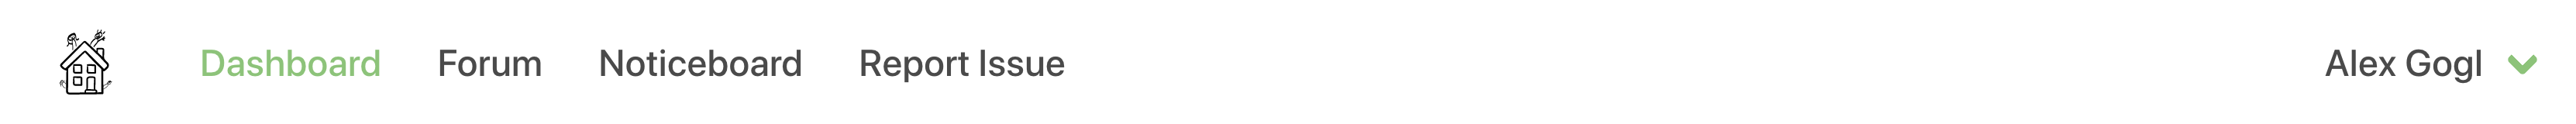
\includegraphics[width=\linewidth]{navbar}
  \end{center}
  \caption{Navbar}
  \label{fig:navbar}
\end{figure}


\subsection{Search Bar \& Create Button}
The search bar and the create button can easily be consoldidated into the same functional component. This way users can search an item and create a new one while the design is kept minimal. This component is defined in a file called "SearchCreateMenu.vue". It builds upon the Bulma "level" element. The search input field is kept on the left, whereas the create button is kept on the right. 

Since this is supposed to be a reusable custom input component it utilizes v-bind to provide a value from the parent component and an event that propagates a value typed by the user up to the parent. This way it is possible to use the "v-model" directive (see \autoref{sub:vmodel}) in order to implement two-way data binding for this component. 

It has several props to make it adaptable for different use cases:

\begin{itemize}
  \item value - used for two way data binding
  \item numberOfItems - shows the number of items currently displayed
  \item pluralTitle - plural description of type of shown items (e.g Thread)
  \item singularTitle - singular description of type of shown items (e.g Threads)
  \item newItem - value of the create button
  \item link - link that will be redirected to upon create button click
\end{itemize}

\begin{figure}[H]
  \begin{center}
  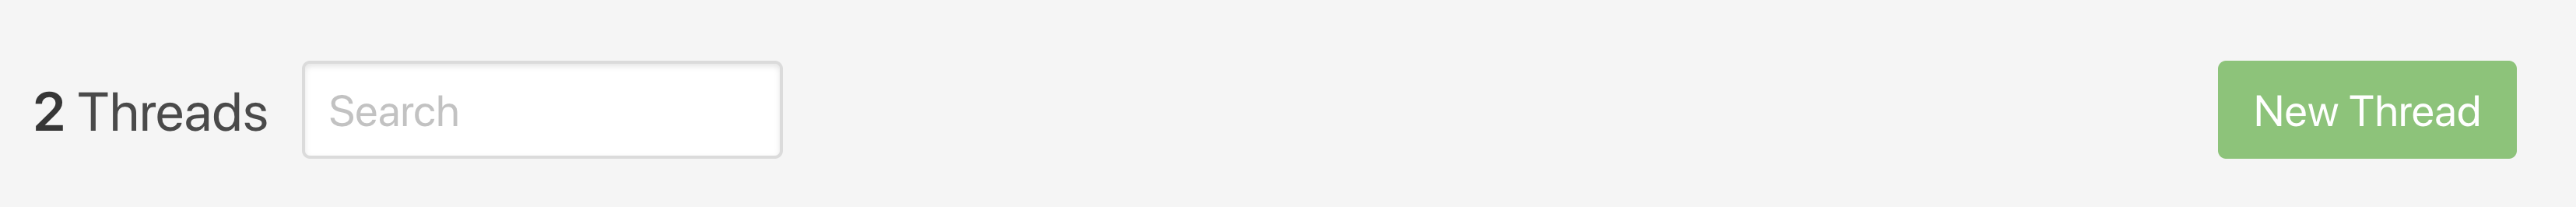
\includegraphics[width=\linewidth]{SearchCreateMenu}
  \end{center}
  \caption{SearchCreateMenu Component}
  \label{fig:searchcreate}
\end{figure}

Usage: The component is used by including it in a page component along with another component that displays a list of items (e.g noticeboard or poll entries). Whenever a user inputs a search string, the v-model property is updated and automatically triggers that a computed property calls a getter method in the store and returns possible items. These possible items are then used to overwrite the list of displayed items.

\subsection{Language Switcher} \label{langswitcher}
The language switcher component has a very simple purpose: instructing the internationalization plugin (detailed description in \autoref{sec:internationalization}) to switch the language. It builds upon Bulmas "select" input element. The component's data object defines an array of languages which are iterated over and displayed as options of the select component. A global property which is provided by the internationalization plugin is encapsulated with "v-model" meaning that whenever a user selects a language which differs from the currently selected one, it is globally updated. Whenever the language is changed, the Vue directive "v-on" makes sure that the function "storeLocale" is called which sets a Cookie in the browser which saves the selected language.

\begin{figure}[H]
  \begin{center}
  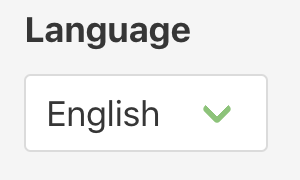
\includegraphics[height=0.8in]{langswitcher}
  \end{center}
  \caption{LangSwitcher Component}
  \label{fig:langswitcher}
\end{figure}

Usage: This component can be used as in a standalone way wherever needed. It is shown on the login page to provide a way of changing languages before a user even uses the application and on the profile page where a user can change preferences.


\subsection{House Switcher}
The House Switcher component works very similar to the Language Switcher component. A select element shows all available houses as options. The user can choose a house and behind the scenes a store mutation is called which changes the active house id in state. This is implemented with a so called "computed setter" - a computed property which in addition to returning cached results, is also capable of "setting" a value. \autoref{computedsetter} depicts how this is implemented: the get function of the computed property returns a cached version of the current house id, the set function updates the id in store and subsequently dispatches an action which repopulates the store with data from the newly selected house's data. The computed property "currentTenement" is then used with v-model which as described earlier is based on the input event and value prop. Vue recognizes when the select element emitts an input event and automatically runs the set function. \newline 

\begin{lstlisting}[caption=Computed Setter, captionpos=b, style=htmlcssjs, label=computedsetter]{Computed Setter}
  computed: {
    currentTenement: {
      get() {
        return this.$store.state.tenement.id;
      },
      set(id) {
        this.$store.commit("tenement/UPDATE", { id });
        this.$store.dispatch("tenement/changeTenement");
      }
    }
  }
\end{lstlisting}

\begin{figure}[H]
  \begin{center}
  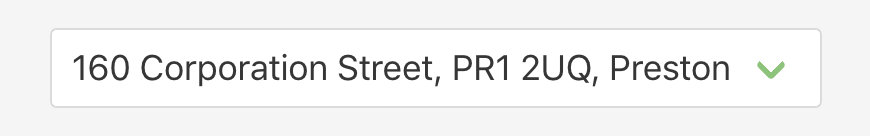
\includegraphics[height=0.8in]{houseswitcher}
  \end{center}
  \caption{ChangeTenement Component}
  \label{fig:langswitcher}
\end{figure}

Usage: Similiar to the Language Switcher Component it can be included in any parent component. It is shown on the main page of the application where the dashboard is located to allow for easy traversal through a user's assigned houses.

\section{Noticeboard}
As defined in \autoref{sub:noticeboardui} the noticeboard page shows a list of all noticeboard entries associated with a house, which are searchable by using the input field of the search bar. The identified elements are a list of all entries, a single entry, and a form for both creating and editing entries which is accessible when clicking the create button.

The composition of these elements are as following:

\begin{itemize}
  \item Noticeboard Page > SearchCreateMenu.vue , BoardList.vue
  \item BoardList.vue > multiple BoardItem(s).vue
  \item Noticeboard Create/Edit Page > CreateBoard.vue
\end{itemize}

* The symbol ">" is read as "is composed of", every page contains the Navbar component

A single noticeboard item is built with the Bulma "tile" component (see \href{https://bulma.io/documentation/layout/tiles/}{Bulma Tile Documentation}). The props of this component are: id, owner, title, content and size. Additionally, a computed property checks if the size prop is passed, if not, the size is calculated depending on the length of the content in terms of characters. The returned string value is a Bulma class which dictates how many rows an element should fill and is added as a dynamic class to the root div element of the component. The "v-if" directive conditionally hides or shows an "edit" anchor tag which links to the edit site of this specifc entry. It does that by comparing the user id saved in store to the owner id which is passed as a prop.

The list containing multiple items defines a prop "boards" of type array which is passed from the page to the list component. It then iterates over this list with "v-for" and passes the specific data of the respective entry to a single item.

The page is composed of a Search Bar and a list of noticeboard entries. The entries are populated by making a request to the API when the page component's mounted lifecycle state is reached.

\begin{figure}[H]
  \begin{center}
  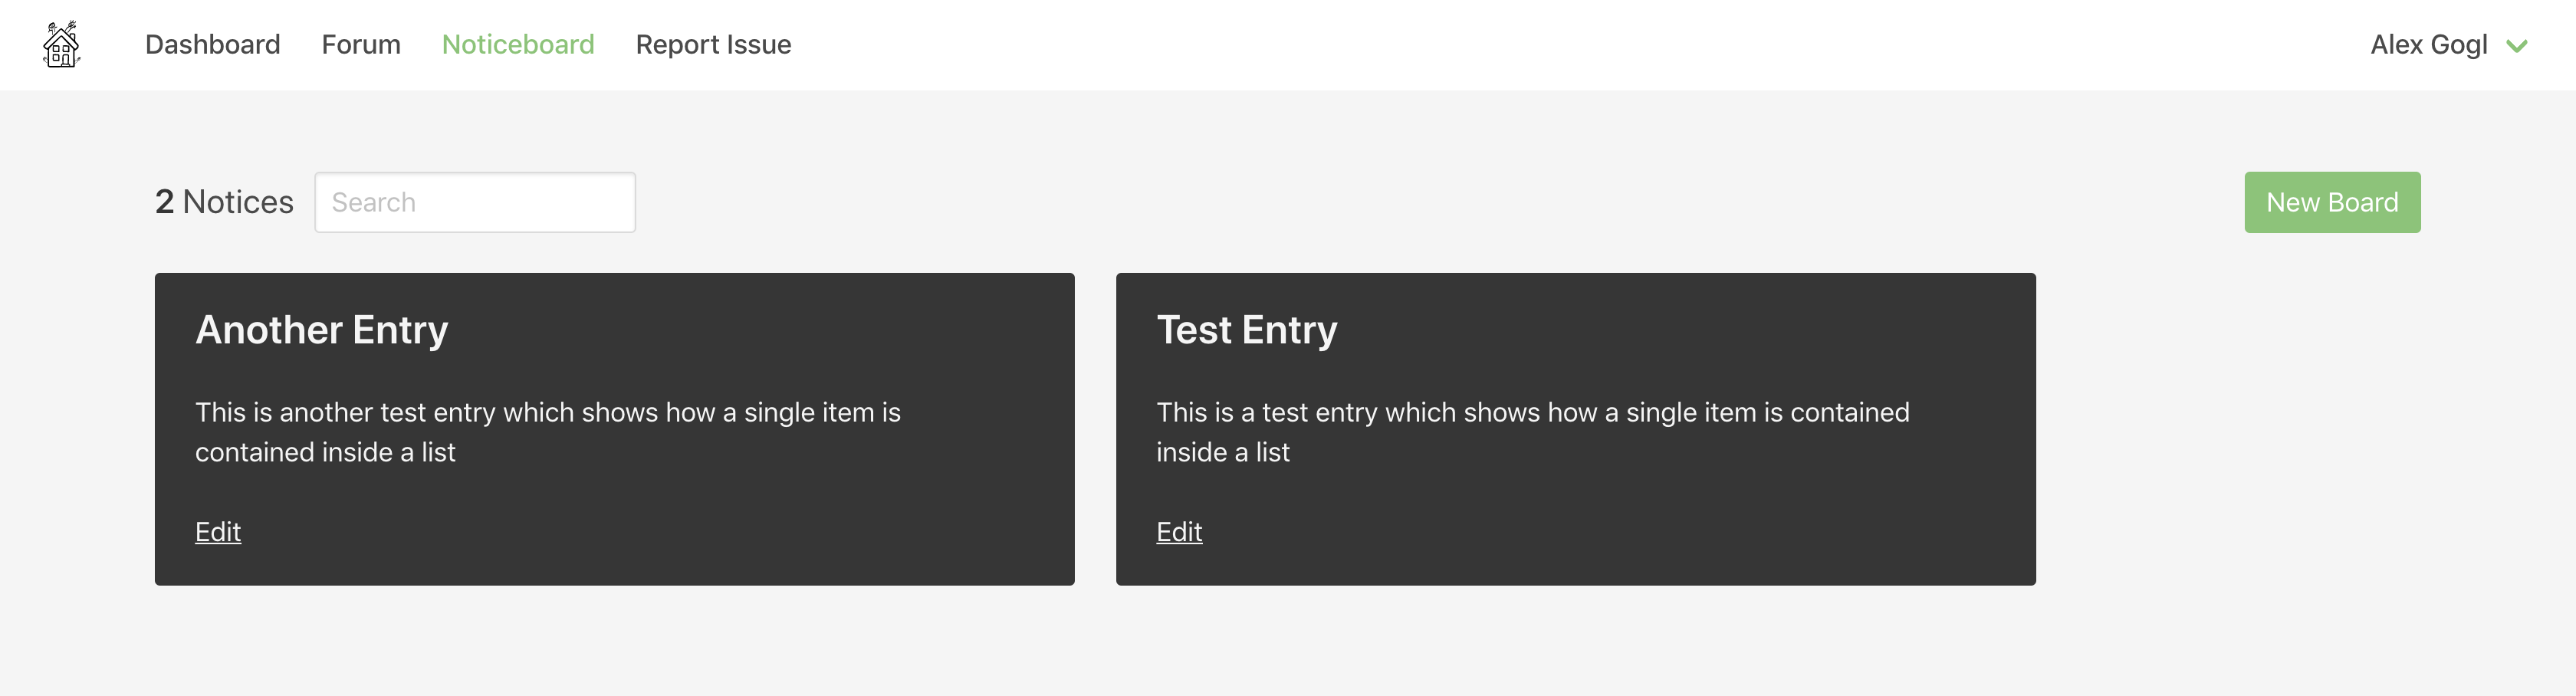
\includegraphics[width=\linewidth]{noticeboardpage}
  \end{center}
  \caption{Noticeboard Page}
  \label{fig:langswitcher}
\end{figure}

\section{Forum}
The Forum page contains a list of all threads associated with a house that are searchable with a Search Bar. When a user clicks on a thread a detail-view is opened which shows the thread in a more detailed manner along with comments and provides a form for creating a new comment.

The composition of components that are related to the Forum are as following:

\begin{itemize}
  \item Forum Page > SearchCreateMenu.vue, ThreadList.vue
  \item ThreadList > multiple ThreadItem(s).vue
  \item Thread Detail Page > ThreadDetail.vue, CommentList.vue, CreateComment.vue
  \item CommentList.vue > multiple CommentItem(s).vue
  \item Thread Create/Edit Page > CreateThread.vue
\end{itemize}

The ThreadList and ThreadItem components are structured like the BoardList and BoardItem components, but use different props and have a different design. An important distinction however, is that ThreadItem components contain a link that redirects to the detail view of the thread. In Nuxt's file structure, subfolders in the pages folder prefixed with underscore are treated differently than normal pages: the router instance is instructed to allow requests to a site with dynamic parameters. E.g. the page folder structure for the thread detail view is as following: "pages/blackboard/\_id". When the application is accessed on \url{https://hausversammlung.at/blackboard/id-of-entry}, the thread detail page does two things in order to show the contents of a specific thread: it checks if thread items exists in the store and if not requests them during the mounted lifecycle state and then retrieves the id parameter of the url to lookup the thread item with that specific id in store (see \autoref{boardentrylookup}). In the store a getter called "getBoardByID" takes the id as a parameter, finds the associated thread in store and returns it. \newline

\begin{lstlisting}[caption=Retrieving Board Entry from Store, captionpos=b, style=htmlcssjs, label=boardentrylookup]{Retrieving Board Entry from Store}
computed: {
  board() {
    return this.$store.getters["blackboard/getBoardByID"](
      this.$route.params.id
    );
  }
}
\end{lstlisting}

\autoref{fig:threaddetail} shows the rendered detail page of a thread item.

\section{Polls}
Polls are a somewhat complicated topic. When a proprietor votes for an option a request needs to be sent to the API and the Poll's UI has to be updated to prevent an addtional option vote. The API however, does not return data which could be used on its own, client-side modification has to occur. As the pages Noticeboard, Forum, Polls and Issues share similar structure and functionality (searching items, creating items, displaying a list of items, populating state) these will not be discussed anymore. Instead, this section aims to describe how a Poll's UI is updated and what data has to be transformed in order to do so.

When voting for a poll option, the Poll Item component emitts an event with the id of the voted option. The Poll List component propagates this id up to the Poll List component which is responsible for dispatching a store action which makes a request to the API. The API then however only returns information on what option was voted on and who voted on it (see \autoref{apidatavoting}). The Poll Item component defines a prop "showResults" which when set to true prevents the user from voting again and shows the results of the poll. The difficulty lies in matching "poll\_answer\_option" to a specific poll. \newline

\begin{lstlisting}[caption=Data returned from API after vote, captionpos=b, style=htmlcssjs, label=apidatavoting]{Data returned from API after vote}
  {
    id: "0aea27f2-4fb6-11e9-9ed5-02420a000613",
    owner: "f85bd1f6-4a44-11e9-9ed5-02420a000613",
    poll_answer_option: "69a0e2e0-4f2a-11e9-9ed5-02420a000613"
  }
\end{lstlisting}

The solution is to iterate over every poll and to compare every option id "option.id" to a parameter "pollOptionId". If the pollOptionId matches any option.id the Poll's showResults prop can be set to true. Additionally, the total number of votes is incremented. This is achieved by using the JavaSript some() method in a nested manner that tests whether at least one element in the array passes a test implemented by a provided function. \autoref{addvote} depicts the corresponding code.

Another and more complicated problem is that when the Polls page is initially acessed, a refresh of the data is requested as desribed in \autoref{statepopulation} but the API only returns a list of polls, a list of options associated with a poll ("poll\_answer\_options") and a list of options that were voted on and are associated with a poll ("poll\_given\_answers"). \autoref{fig:pollsbefore} shows the raw data that is returned before any change is made to the data structure. Similarly to the previous problem, the client side needs to make certain changes to the data structure to make polls non-interactible when a user has already voted for that option. \autoref{updatevotes} shows the mutation that is called that makes these changes after all polls are retrieved. \newline

\begin{lstlisting}[caption=Update Votes, captionpos=b, style=htmlcssjs, label=updatevotes]{Update Votes}
  UPDATE_VOTES(state, userId) {
  const pollList = [];

  //find all poll_given_answers by userId and add id of answer_option to pollList
  state.polls.filter(o =>
    o.poll_given_answers.some(answer => {
      if (answer.owner === userId) {
        pollList.push(answer.poll_answer_option);
        o.showResults = true;
        return true;
      }
    })
  );

  //iterate over poll_answer_options and check if id is in pollList
  //update if it is
  state.polls.filter(o =>
    o.poll_answer_options.some(option => {
      if (pollList.includes(option.id)) {
        option.selected = true;
      }
    })
  );
}
};
\end{lstlisting}

In lines 5 to 13 every poll item and their respective voted items is iterated over and checked if a vote's owner matches the user id of the application's user. If it does, this vote is added to an array "pollList" and the whole poll is instructed to show the results with "o.showResults = true". What is left now is to tell the poll which item the application's user has voted on and to render it accordingly. In lines 17 to 23 all polls are iterated over and it is checked if any vote's id is included in the pollList array and if it is, this specific poll option is set as selected. \autoref{fig:pollsafter} shows the data structure of polls after this update.

To visually illustrate what is meant, \autoref{fig:pollitem} shows the rendered Poll Item Component with the "Yellow" option set as the selected item and the poll being in "showResults" state.

\begin{figure}[H]
  \begin{center}
  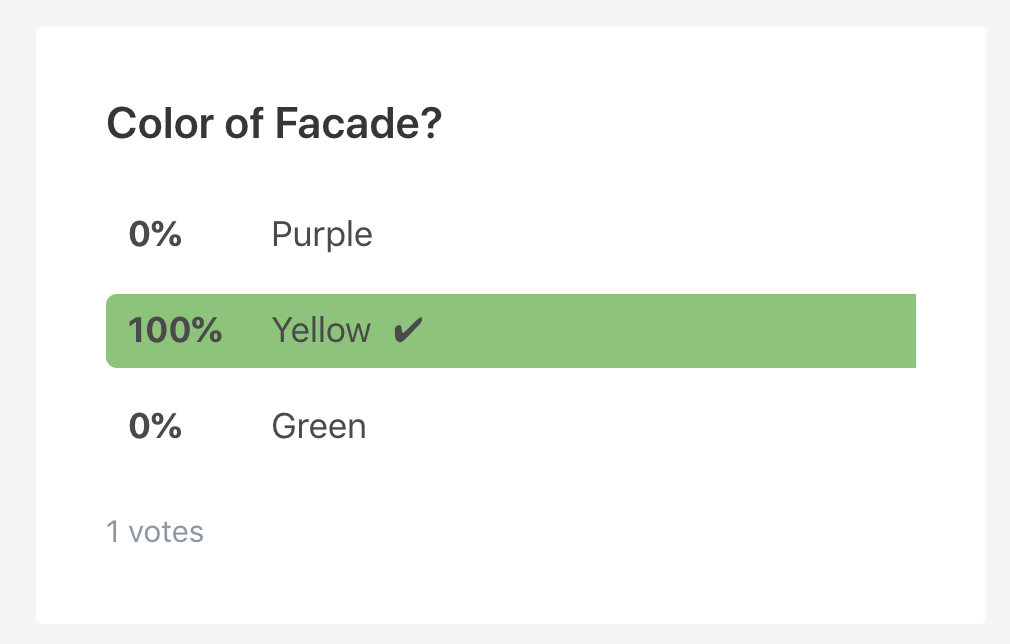
\includegraphics[height=1.5in]{pollitem}
  \end{center}
  \caption{Poll Item}
  \label{fig:pollitem}
\end{figure}

\section{Issue Log System}
The Issues page shows maintenance or house related issues. To give users a quick overview of all existing issues, a table was chosen to show them. More information regarding tables in Bulma is available at \url{https://bulma.io/documentation/elements/table/}. The component structure is similar to the other pages: \newline

\begin{itemize}
  \item Issue Page > SearchCreateMenu.vue, IssueTable.vue
  \item Create/Edit Issue Page > CreateIssue.vue
\end{itemize}

The only distinction is the type of data which is shown and how it is displayed: issues. A table shows Reference, Date,  Type, Location, Title and Status which can be sorted in ascending or descending order. Additionally, users can edit issues if they are their owners, a button is shown accordingly. The API currently does not support an issue state being changed by facility management even though it is stated in the requirements. This functionality is therefore not implemented on the client side. \autoref{fig:issuetable} shows the rendered Issue page.

\begin{figure}[H]
  \begin{center}
  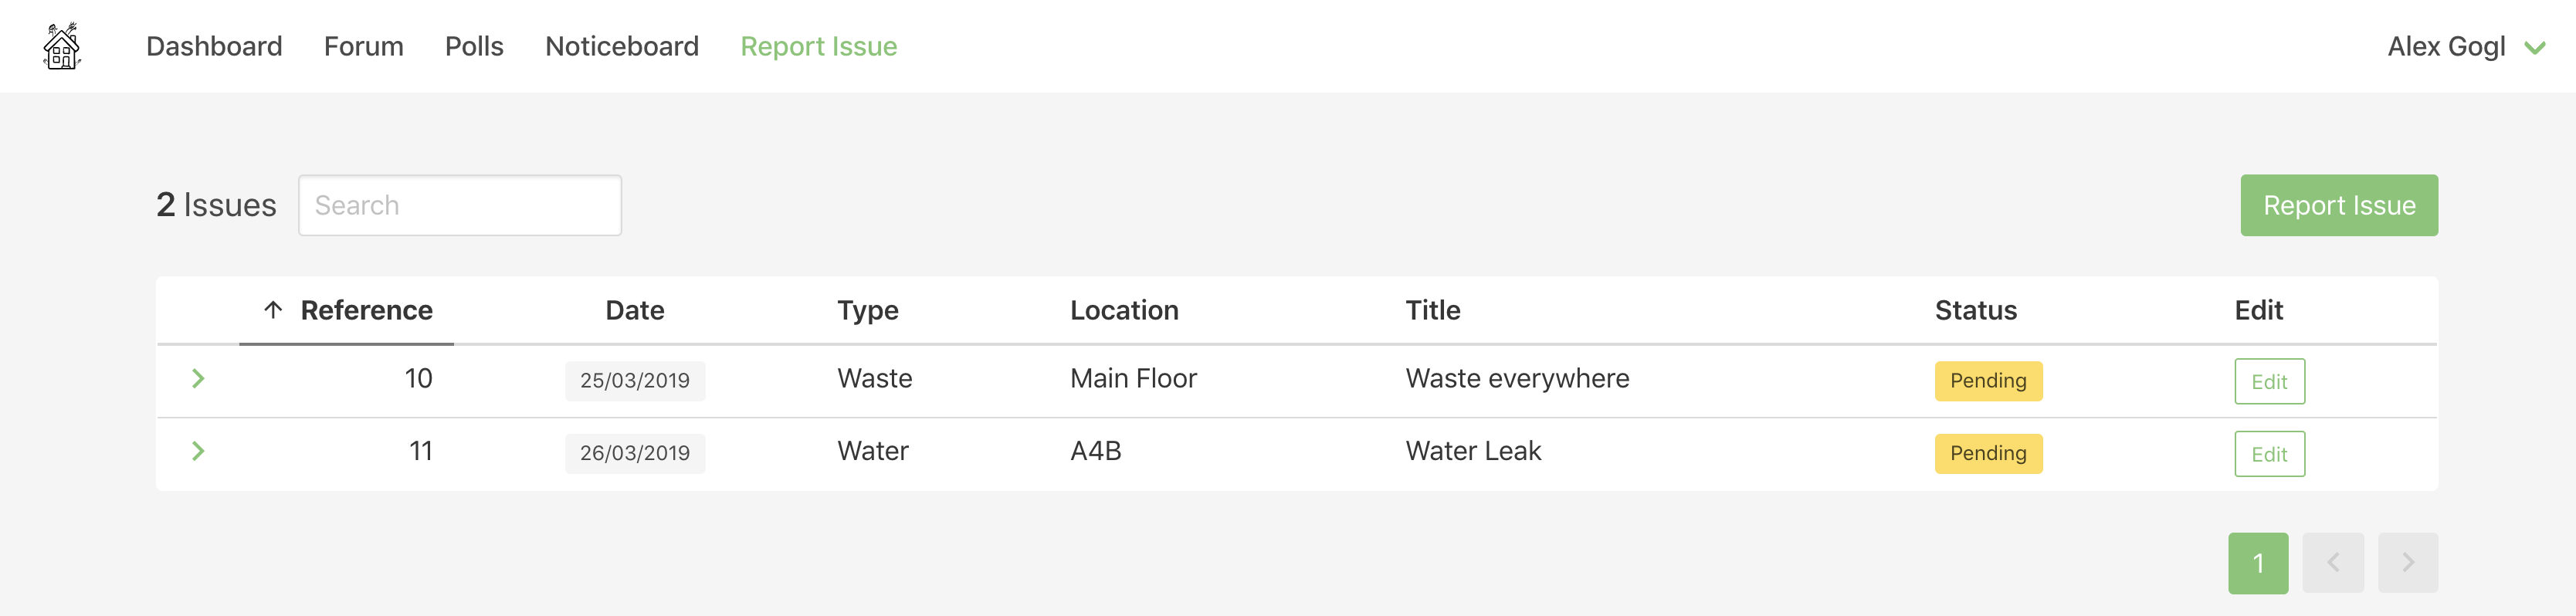
\includegraphics[width=\linewidth]{issues}
  \end{center}
  \caption{Issue Page}
  \label{fig:issuetable}
\end{figure}

\section{Adding a house}
As required by the user stories (see \autoref{subsub:userstorieshouse}) and defined by the use case flows (see \autoref{usecases:house}), a house should either be creatable by a user or they should be able to accept an invitation. Additionally, they should be able to send new invitations. Implementation is relatively straightforward, for each use case one component exists that provides a form. After the user inputs the required data and submits the form, the API handles the rest. On the client-side the new house is added to an array of houses along with basic information. The user can then switch houses by using the Change House component. \autoref{fig:addhouse} shows the rendered implemenation of a form where a new house can be added, \autoref{fig:acceptinvite} a form to accept an existing invitation and \autoref{fig:sendinvite} a form to send invitations.

Sending an invitation requires an email address which will be sent instructions to add an existing house to the user's account. More specifically, the email contains a link with a special id as a query parameter which is retrieved by the application to pre-populate the invitation form.  

\section{Dashboard}
The dashboard which is shown on the main page is populated with data that exists in store. The most recent polls, threads and noticeboard entries are shown. Additionaly, metrics on number of users, squaremeters of a user, number of houses a user is associated with and nubmer of issues associated with this house are displayed. \autoref{fig:dashboard} illustrates an example dashboard.

\begin{figure}[H]
  \begin{center}
  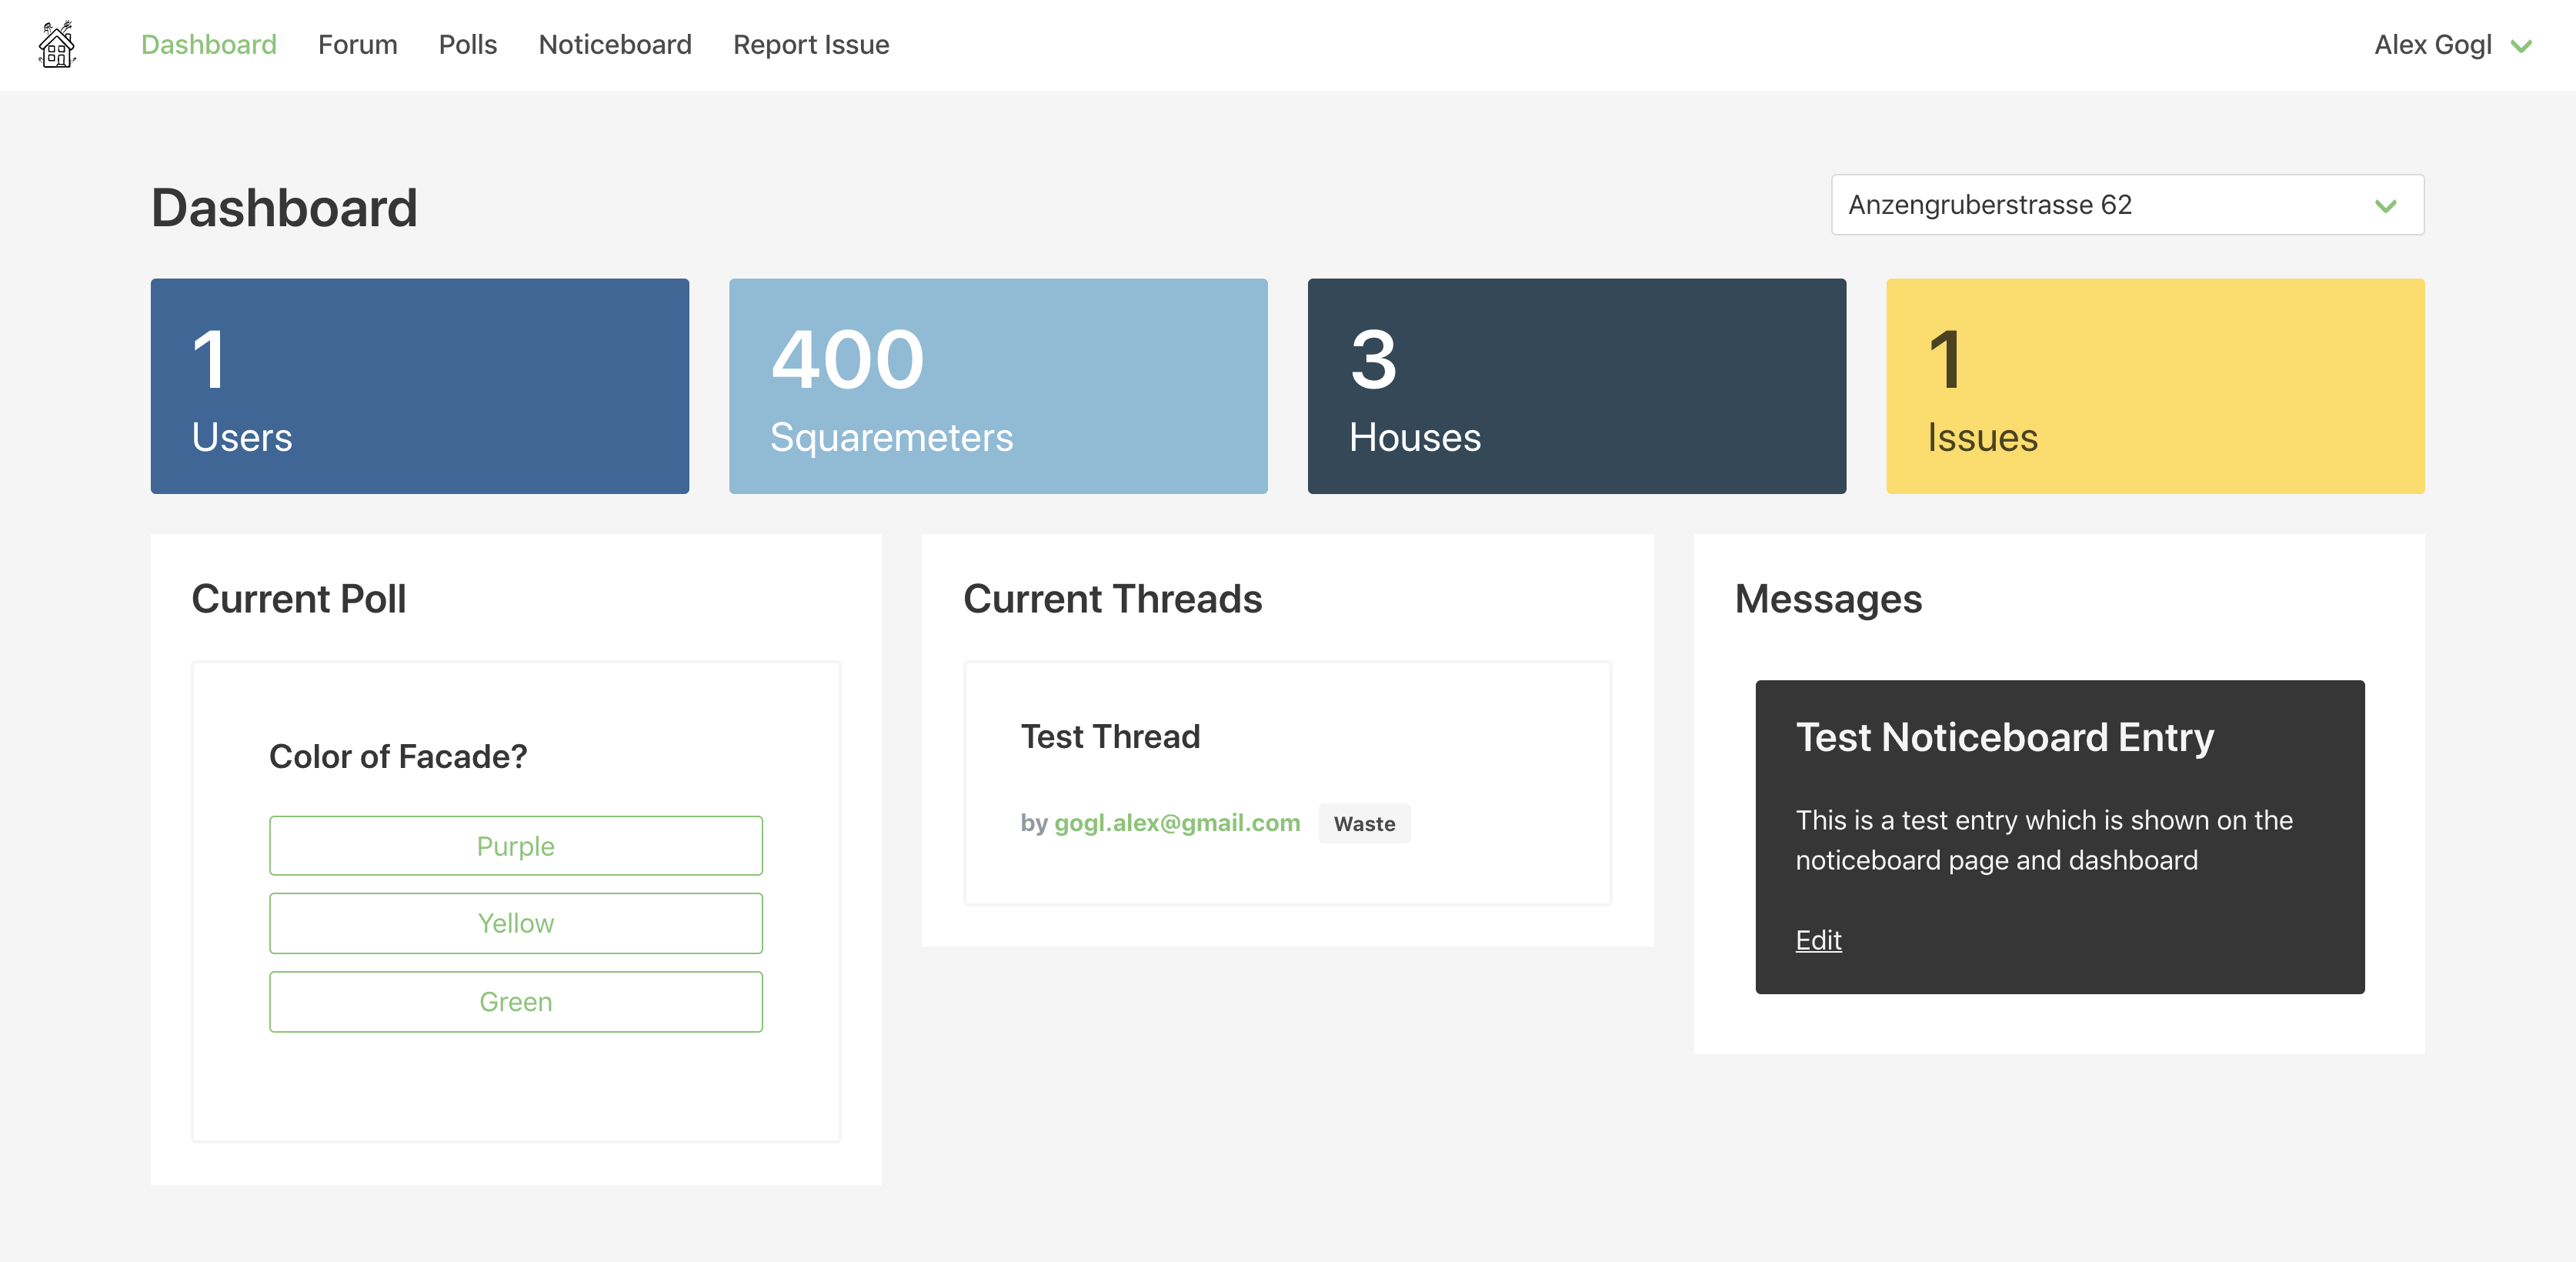
\includegraphics[width=\linewidth]{dashboard}
  \end{center}
  \caption{Dashboard Page}
  \label{fig:dashboard}
\end{figure}

As already mentioned, the data used to populate the dashboard with, is retrieved from the store. This happens by using vuex store functions, more specifically: getters, as described in \autoref{vuex}. 

\section{Internationalization} \label{sec:internationalization}
As the primary target market of the application is Austria, where German is spoken but English is also commonly used, two languages have to be offered. This is achieved by a third-party package called \href{https://github.com/kazupon/vue-i18n}{vue-i18n} which is added as a custom Nuxt plugin. Instead of hardcoding the labels, descriptions, titles and other strings into the application, two language files "de-AT.json" and "en-US.json" are created which define key value pairs of a strings and their translations. The plugin injects a method "\$t" into every component which can be used to retrieve the appropriate value. \newline

\begin{lstlisting}[caption=Data returned from API after vote, captionpos=b, style=htmlcssjs, label=apidatavoting]{Data returned from API after vote}
  //hardcoded
  <h1 class="title is-3">Create a House</h1>
  //translation retrieved with injected method
  <h1 class="title is-3">{{ $t("house.newHouse") }}</h1>
\end{lstlisting}

The package also injects the global property "\$i18n.locale" into the root Vue instance which represents the currently selected language. For example if German was selected, the property's value would be "de". This property is used by the computed setter described in \autoref{langswitcher} to globally change the language.

\section{Client-side Validation}
Client-side validation is mainly used as a means of usability. It is possible for a user with malicious intent to bypass any client side validation mechanism and applies to every frontend application. Thorough server-side validation can never be replaced. However, the usability of an application is drastically improved if users get instantaneous feedback on their input. To achieve this, another third party package \href{https://baianat.github.io/vee-validate/}{VeeValidate} is used which uitilizes JavaScript to validate input. Another solution would be to rely on the standard HTML validation capabilites of every modern browser. With HTML validation, simple input like emails, strings that should have a min or max character value or even input based on regexes can be validated. However, more sophisticated checks cannot be implemented: an example which also applies to this application is that one inputs's value should not be greater than anothers. In this case, such a check is used to make sure that a user does not supply a greater value of their squaremeters than a house has in total during the "add house" process. In practical terms, the plugin injects the additional directive "v-validate" which takes either an object or string containing the rules as a paremeter. \newline


\begin{lstlisting}[caption=v-validate usage, captionpos=b, style=htmlcssjs, label=vvalidate]{v-validate usage}
<BInput
  v-model="share"
  v-validate="{
    required: true,
    max_value: sum_shares
  }"
  type="number"
/>
\end{lstlisting}


\autoref{vvalidate} depicts a concrete usage example of how it is achieved that one value cannot be greater than another user-supplied value. 

\section{Error Handling}
The application has several sources where errors can occur. Naturally, these errors should be dealt with gracefully while providing error explanations to the user. The by far biggest source of error is when a request to the API is made and an error is returned. This can have various reasons such as a timeout exception, failed validation or non existing records. The importance lies in dealing with these errors in a manner that leaves the application still interactive while adhering to Nielsen's "Visibility of System Status" principle. This is achieved with a pattern of catching and rethrowing errors, whereby these are dealt with in the most appropriate place. For example it is not very sensible for the store to initiate showing an error message, rather, the component which initially called the action from store that made the request should deal with it, because at this level there are much more options available. As most API requests are made from the store, a choice was made to catch and rethrow so components can take care of them. This not only improves maintainability but also makes for a more loosely coupled system. \autoref{storerethrow} depicts a pseudo login store action which rethrows errors when they occur. The code in \autoref{componenterrorcatch} catches these errors and displays an error message accordingly. \newline

\begin{lstlisting}[caption=Store Action Error Rethrow, captionpos=b, style=htmlcssjs, label=storerethrow]{Store Action Error Rethrow}
  async login() {
    try {
      await pseudoApiRequest();
    } catch (error) {
      throw error;
  }
\end{lstlisting}

To display error messages, another third-party package \href{https://github.com/shakee93/vue-toasted}{Vue Toasted} is used. It is set up in way that also makes error messages bilingual. The associated configuration can be found in the file plugins/toasted.js file. \newline

\begin{lstlisting}[caption=Catch Error in Component, captionpos=b, style=htmlcssjs, label=componenterrorcatch]{Catch Error in Component}
  async login(authData) {
    try {
      await this.$store.dispatch("auth/login");
    } catch (error) {
      this.$toasted.global.my_error({
        message: this.$t("toasts.loginFailed")
      });
  }
\end{lstlisting}

Another noteworthy point is that throughout the application async/await is utilized which according to the JavaScript documentation is used to "... to simplify the behavior of using promises synchronously and to perform some behavior on a group of Promises" \cite{JavaCriptDoc:online}. In addition, it makes the code cleaner and more comprehensible.
